\subsection{(10\%) Bezier motion (2012 No. 6)}
Scalars in bezier curves are found by factoring Bernstein polynomials:
\begin{itemize}
    \item BL = ((1 - t) + t) L for a bezier curve with L + 1 control points.
\end{itemize}

An object is moved along a bezier curve with 4 control points.
\begin{itemize}
    \item P1 = (15, 5, 2)
    \item P2 = (10, 2, 2)
    \item P3 = (5, 7, 2)
    \item P4 = (0, 0, 2)
\end{itemize}

The motion should start 4 seconds after the program starts and it should end 20 seconds later, 24 seconds after the program starts.

\subsubsection{Where is the object's center 19 seconds after the program started?}

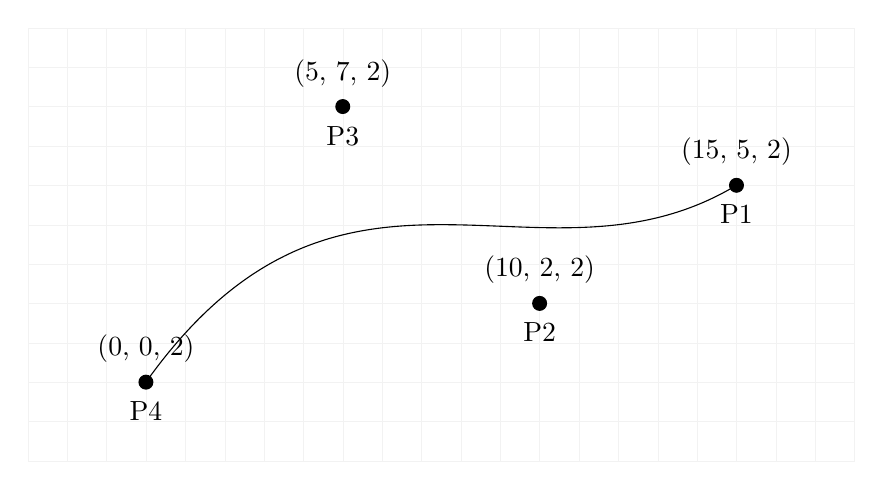
\begin{tikzpicture}[scale=0.5]
    \draw[step=1.0cm, gray!10, ultra thin](-3, -2) grid (18, 9);
    \draw 
        (15, 5) .. controls (10, 2) and (5, 7) .. (0, 0);
    
    \filldraw (15, 5) circle (5pt) node[label={below:P1}, label={above:(15, 5, 2)}]{} {};
    \filldraw (10, 2) circle (5pt) node[label={below:P2}, label={above:(10, 2, 2)}]{} {};
    \filldraw (5, 7) circle (5pt) node[label={below:P3}, label={above:(5, 7, 2)}]{} {};
    \filldraw (0, 0) circle (5pt) node[label={below:P4}, label={above:(0, 0, 2)}]{} {};
\end{tikzpicture}

$ t_{start} = 4$

$ t_{duration} = 20$

$ t_{now} = 19$

$ delta = \frac{t_{now} - t_{start}}{t_{duration}} = \frac{15}{20} = \frac{3}{4} $

\newpage

\textbf{Iteration 1:}

$ 
    \vec{P1_1} 
= 
    lerp\left(P1_0, P2_0, delta\right)
=
    lerp\left(
        \veciii{15}{5}{2}, 
        \veciii{10}{2}{2},
        \frac{3}{4} 
    \right)
=
    \veciii{11.25}{2.75}{2}
$

$ 
    \vec{P2_1} 
= 
    lerp\left(P2_0, P3_0, delta\right)
=
    lerp\left(
        \veciii{10}{2}{2}, 
        \veciii{5}{7}{2},
        \frac{3}{4} 
    \right)
=
    \veciii{6.25}{5.75}{2}
$

$ 
    \vec{P3_1} 
= 
    lerp\left(P3_0, P4_0, delta\right)
=
    lerp\left(
        \veciii{5}{7}{2},
        \veciii{0}{0}{2}, 
        \frac{3}{4} 
    \right)
=
    \veciii{1.25}{1.75}{2}
$

\textbf{Iteration 2:}

$ 
    \vec{P1_2} 
= 
    lerp\left(P1_1, P2_1, delta\right)
=
    lerp\left(
        \veciii{11.25}{2.75}{2}
        \veciii{6.25}{5.75}{2}
        \frac{3}{4} 
    \right)
=
    \veciii{7.5}{5}{2}
$


$ 
    \vec{P1_2} 
= 
    lerp\left(P1_1, P2_1, delta\right)
=
    lerp\left(
        \veciii{6.25}{5.75}{2}
        \veciii{1.25}{1.75}{2}
        \frac{3}{4} 
    \right)
=
    \veciii{2.5}{2.75}{2}
$

\textbf{Iteration 3:}

$ 
    \vec{P1_3}
= 
    lerp\left(P1_2, P2_2, delta\right)
=
    lerp\left(
        \veciii{7.5}{5}{2}
        \veciii{2.5}{2.75}{2}
        \frac{3}{4} 
    \right)
=
    \veciii{3.75}{3.3125}{2}
$

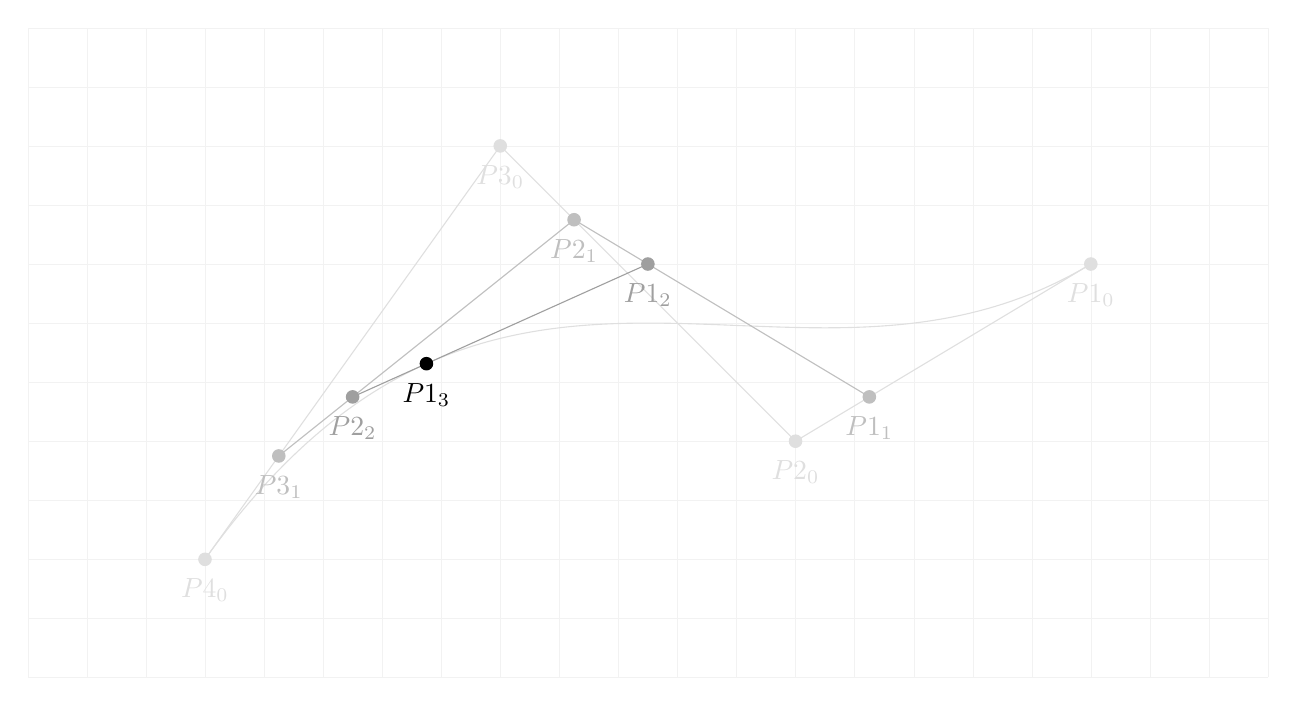
\begin{tikzpicture}[scale=0.75]
    \draw[step=1.0cm, gray!10, ultra thin](-3, -2) grid (18, 9);
    \draw[gray!25] (15, 5) .. controls (10, 2) and (5, 7) .. (0, 0);
    
    % Iteration 1
    \draw[gray!25] (15, 5) -- (10, 2) -- (5, 7) -- (0, 0);
    \filldraw[gray!25] (15, 5) circle (3pt) node[label={below:$P1_0$}]{} {};
    \filldraw[gray!25] (10, 2) circle (3pt) node[label={below:$P2_0$}]{} {};
    \filldraw[gray!25] (5, 7) circle (3pt) node[label={below:$P3_0$}]{} {};
    \filldraw[gray!25] (0, 0) circle (3pt) node[label={below:$P4_0$}]{} {};
    
    % Iteration 2
    \draw[gray!50] (11.25, 2.75) -- (6.25, 5.75) -- (1.25, 1.75);
    \filldraw[gray!50] (11.25, 2.75) circle (3pt) node[label={below:$P1_1$}]{} {};
    \filldraw[gray!50] (6.25, 5.75) circle (3pt) node[label={below:$P2_1$}]{} {};
    \filldraw[gray!50] (1.25, 1.75) circle (3pt) node[label={below:$P3_1$}]{} {};
    
    % Iteration 3
    \draw[gray!75] (7.5, 5) -- (2.5, 2.75);
    \filldraw[gray!75] (7.5, 5) circle (3pt) node[label={below:$P1_2$}]{} {};
    \filldraw[gray!75] (2.5, 2.75) circle (3pt) node[label={below:$P2_2$}]{} {};
    
    % Result:
    \filldraw (3.75, 3.3125) circle (3pt) node[label={below:$P1_3$}]{} {};

\end{tikzpicture}

The object's center is at $ \veciii{3.75}{3.3125}{2} $ when $ t = 19 $. The calculation took 3 iterations.

\rule{\textwidth}{0.25mm}
This was actually fun to calculate and draw. I have to say that these hand-ins have had a really good learning effect for me. (Let's hope that the results are also correct.) I'm almost sad that this is the last one.

But all good things must end at one point. Thank you very much!